\begin{titleDef}{Normen}
\label{norm}
Eine Norm ist eine Abbildung $\lVert \cdot\rVert:V\to\mathbb{R}^+_0,\ x\mapsto\lVert x\rVert$ für einen Vektorraum $V$ für die gilt:\\
Für alle $x,y\in V,\lambda\in\mathbb{R}$:
\begin{enumerate}[label=(\arabic*)]
	\item \textbf{Definitheit:}$\lVert x\rVert=0\Leftarrow x=0$
	\item \textbf{Homogenität:}$\lVert \lambda x\rVert=\lvert\lambda\rvert\lVert x\rVert$
	\item \textbf{Dreiecksungleichung:}$\lVert x+y\rVert\leq\lVert x\rVert+\lVert y\rVert$
\end{enumerate}
Die klassischen Beispiele sind die $\ell_1,\ell_2,\ell_\infty$-Normen.
\begin{enumerate}[label=(\arabic*)]
	\item \textbf{$\ell_1$:}$\lVert x\rVert_1=\sum_{i=1}^{n}\lvert x_i\rvert$        
	\item \textbf{$\ell_2$:}$\lVert x\rVert_2=\sqrt{\sum_{i=1}^{n}x_i^2}$   
	\item \textbf{$\ell_\infty$:}$\lVert x\rVert_\infty=\max\{x_1,\ldots,x_n\}=\max\limits_{1\leq i\leq n}x_i$                   
\end{enumerate}
\begin{figure}[h]
	\centering
	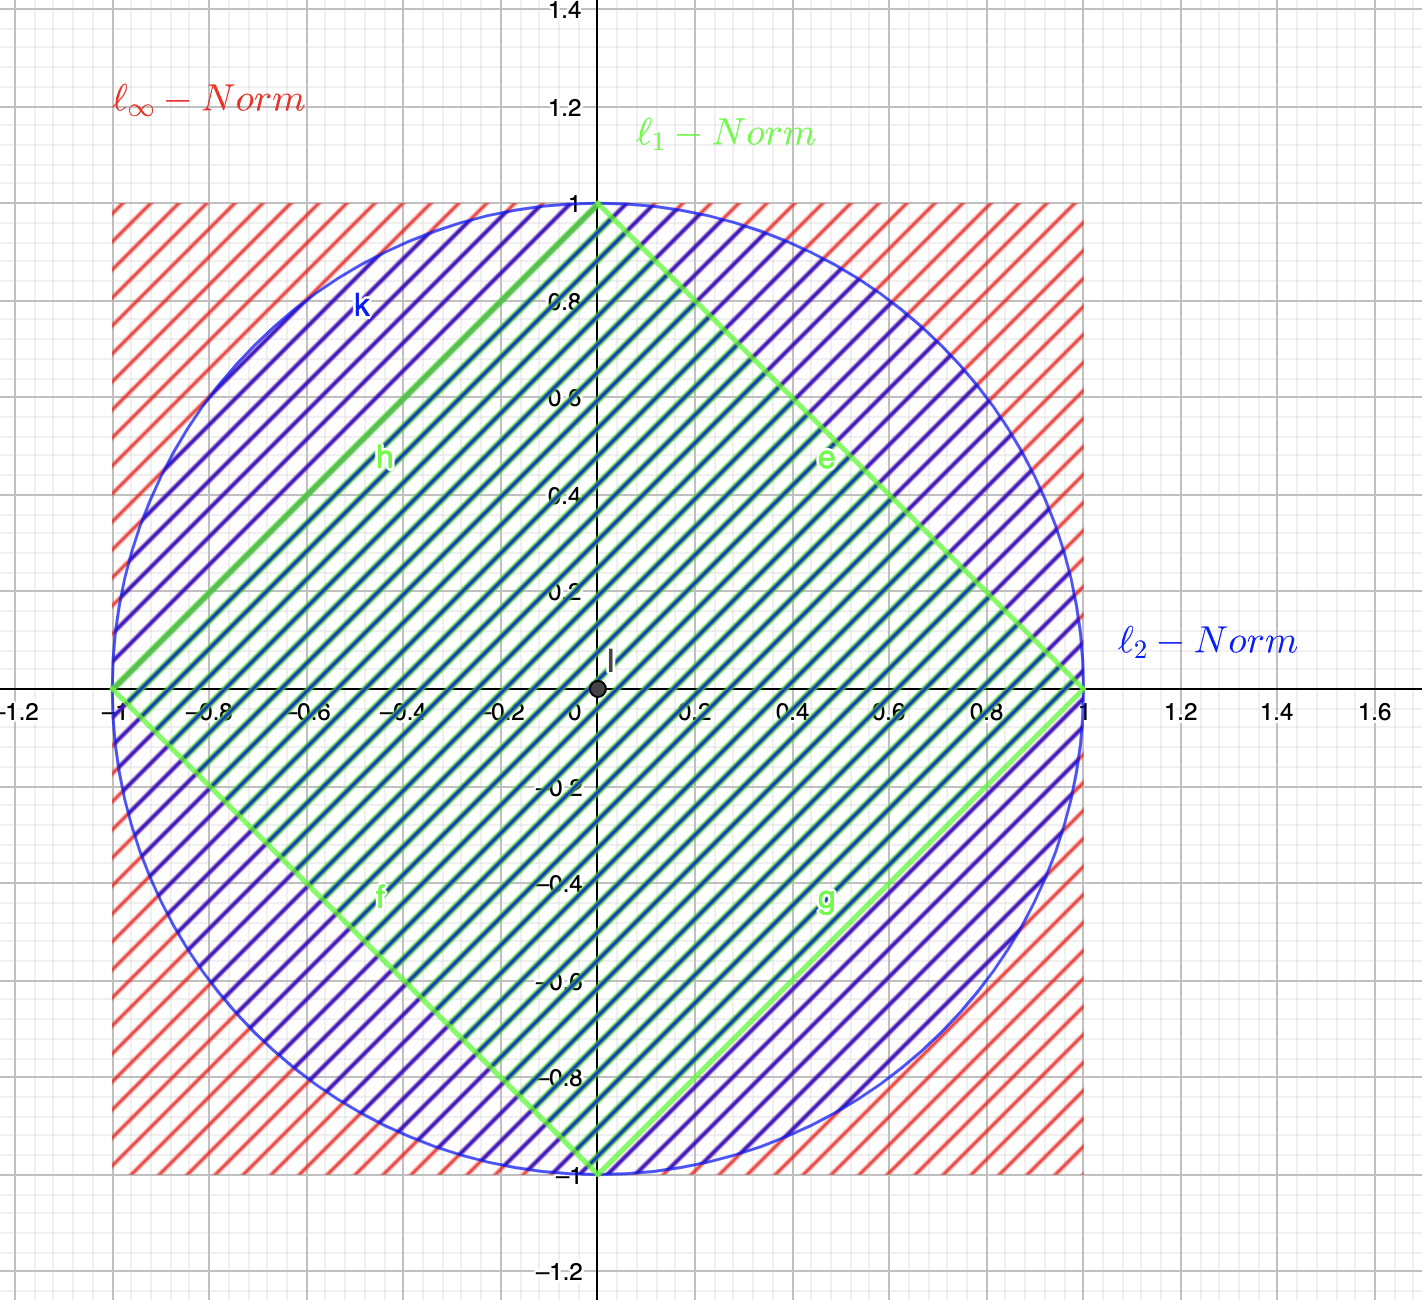
\includegraphics[width=\linewidth]{Bilder/Norms}
	\label{normbild}
\end{figure}\par
\end{titleDef}

\begin{titleDef}{Metrik}
\label{Metrik}
Sei X eine Menge. Eine Abbildung $d:X\times X:\to \mathbb{R}_{\ge0}$ ist eine \textbf{Metrik}, falls für alle $x,y,c\in X$ gilt:
\begin{enumerate}
    \item positiv definit: $d(x,y)=0\Leftrightarrow x=y$
    \item symmetrisch: $d(x,y)=d(y,x)$
    \item Dreickesungleichung: $d(x,z)\le d(x,y)+d(y,z)$
\end{enumerate}
\end{titleDef}

\begin{titleDef}{Abstandserhaltend}
\label{abstandserhaltend}
Seien $(X,d_X),(Y,d_Y)$ \hyperref[MetrischerRaum]{metrische Räume}. Eine Abbildung $f:X\to Y$ heißt abstandserhaltend, falls für alle $x,y\in X$ gilt: $d_Y(f(x),f(y))=d_X(x,y)$
\end{titleDef}

\begin{titleDef}{Isometrie}
\label{Isometrie}
Eine Isometrie ist eine bijektive, \hyperref[abstandserhaltende]{abstandserhaltend} Abbildung.\par
Seien $S,\tilde{S}$ \hyperref[regFlaeche]{reguläre Flächen}. Eine Abbildung $f:S\to\tilde{S}$ heißt \textbf{Isometrie}, wenn $f$ ein \hyperref[diffeomorph]{Diffeomorphismus} zwischen $S$ und $\tilde{S}$ ist und für alle \hyperref[diffFlaechenkurve]{differenzierbaren Kurven} $c:I\to S$ gilt, dass die \hyperref[laengeFlaechenkurve]{Länge der Kurve} unter $f$ invariant ist also $L(f\circ c)=L(c)$.\\
Für die metrischen Räume auf den regulären Flächen $(S,d_S),(\tilde{S},d_{\tilde{S}})$ gilt insbesondere $d_{\tilde{S}}(f(p),f(q))=d_S(p,q)$
\end{titleDef}

\begin{titleDef}{lokale Isometrie}
\label{lokIso}
Eine Abbbildung $f:S\to\tilde{S}$ zwischen \hyperref[regFlaeche]{regulären Flächen} $S,\tilde{S}$ heißt \textbf{lokale Isometrie}, falls für jeden Punkt $p\in S$ eine \offUm $U\subset S$ von p und $V\subset\tilde{S}$ von $f(p)$ existiert, so dass $f$ eingeschränkt auf $U$ eine Isometrie zwischen $U$ und $V$ ist.\par
Sind $S,\tilde{S}$ \hyperref[regFlaeche]{reguläre Flächen} mit \hyperref[parametrisierung]{Parametrisierungen}
$$x:U\to x(U)\subset S\qquad \tilde{x}:U\to \tilde{x}(U)\subset\tilde{S}$$
so dass die \hyperref[fundamentalformEins]{1.Fundamentalform} von $S$ und $\tilde{S}$ in den Punkten $(u,v)\in U$ aus $U$ übereinstimmen, also
$$
	\begin{pmatrix} 
	\mathrm{E}(u,v) & \mathrm{F}(u,v)\\
	\mathrm{F}(u,v) & \mathrm{G}(u,v)
\end{pmatrix} = 
	\begin{pmatrix} 
	\mathrm{\tilde{E}}(u,v) & \mathrm{\tilde{F}}(u,v)\\
	\mathrm{\tilde{F}}(u,v) & \mathrm{\tilde{g}}(u,v)
\end{pmatrix} 
$$
Dann sind $x(U)\subset S$ und $\tilde{x}(U)\subset\tilde{S}$ isometrisch.
\end{titleDef}

\begin{titleDef}{Stetigkeit}
\label{stetig}
Seien $(X,\mathcal{O}_X)$ und $(Y,\mathcal{O}_Y)$ \hyperref[Topologie]{topologische Räume}.\\
Eine Abbildung $f:X\to Y$ heißt \textbf{stetig}, falls die Urbilder von offenen Mengen in Y stets offen sind in X.
$$\text{f stetig} \Leftrightarrow \text{Für alle } V\in\mathcal{O}_Y \text{ ist } f^{-1}=\{x\in X|\ f(x)\in V\}\in\mathcal{O}_X$$\\
Folgende Aussagen sind äquivalent:
\renewcommand{\labelenumi}{(\roman{enumi})}
\begin{enumerate}
    \item f ist stetig
    \item Für alle $x\in X$ gilt:
    $$\forall\varepsilon>0\ \exists \delta=\delta(\varepsilon,x), \text{ so dass } f(B_\delta^X(x))\subseteq B_\varepsilon^Y(f(x))$$
    \item f ist folgenstetig, d.h für alle $x\in X$ gilt
    $$x=\lim_{x\to\infty}x_n \Rightarrow f(x)=\lim_{n\to\infty}f(x_n)$$
\end{enumerate}
Jede stetige Funktion auf einer \hyperref[kompakt]{kompakten Teilmenge} eines \hyperref[Topologie]{topologischen Raumes} hat ein endliches Maximum und Minimum, ist also insbesondere beschränkt.
\end{titleDef}

\begin{titleDef}{Homöomorphismus}
\label{homoemorph}
Eine bijektive Abbildung zwischen \hyperref[Topologie]{topologischen Räumen} $f:X\to Y$ heißt \textbf{Homöomorphismus}, falls $f$ und ihre Umkehrabbildung $f^{-1}$ stetig sind, d.h:
\begin{align*}
    \text{f ist homöomorphismus}&\Longleftrightarrow f\text{ bijektiv und }f,f^{-1}\text{ stetig}\\
    &\Longleftrightarrow U\subseteq X\text{offen}\Longleftrightarrow f(U)\subseteq Y\text{offen}
\end{align*}\\
Damit ist homöomorphismus stärker als stetigkeit weil bei Stetigkeit nur $$f^{-1}(U)\subseteq Y\text{ offen}\Rightarrow U\subseteq X\text{ offen gilt.}$$
Die \hyperref[Topologie]{topologischen Räumen} $X$ und $Y$ heißen \textbf{homöomorph} wenn es einen Homöomorphismus $f:X\to Y$ gibt. Geschrieben $X\simeq Y$.\\
\textbf{Beispiel:}
\listbsp
\begin{enumerate}
    \item Alle abgeschlossenen Intervalle bzgl der \hyperref[stdTopo]{Standard-Topologie} sind homöomorph:
    $$[0,1]\simeq [a,b]\text{ für alle }a<b\in\mathbb{R}$$
    Gleiches gilt für die offenen intervalle $(0,1)\simeq (a,b)$. Ein Homöomorphismus ist gegeben durch $f(t)=a+t(b-a)$
    \item Ganz $\mathbb{R}$ ist bzgl der \hyperref[stdTopo]{Standard-Topologie} homöomorph zu einem offenen Intervall:
    $$\mathbb{R}\simeq(-1,1)\simeq(0,1)$$
    Ein Homöomorphismus ist gegeben durch $f(t)=tanh(t)=\frac{e^{2t}-1}{e^{2t}+1}$
    \item Seien $(X,d_X),(Y,d_Y)$ \hyperref[MetrischerRaum]{metrische Räume} und $f:X\to Y$ eine \hyperref[Isometrie]{Isometrie}. Dann ist $f$ ein Homöomorphismus. Setzte $\varepsilon=\delta$ dann:
    $$d_X(x,y)<\delta \Rightarrow d_Y(f(x),f(y))=d_X(x,y)<\delta=\varepsilon$$
    Also wenn ein Punkt x im \hyperref[balloffen]{Delta-Ball} $B_{\delta}(y)$ um y liegt, dann liegt f(x) im \hyperref[balloffen]{Epsilon-Ball} $B_{\varepsilon}(f(y))$ um f(y) für beliebige x und y. Also $f(B_{\delta}(y))\subseteq B_{\varepsilon}(f(y))$ und damit sind die Bilder von offenen Mengen unter f wieder offen und analog umgekehrt.
    \item \begin{titleDef}{stereographische Projektion}
    \label{stereoproj}
    Sei $S^n=S^n_1=\{x\in\mathbb{R}^{n+1}|\ \lVert x\rVert^2=x_1^2+\dots+x_{n+1}^2=1\}$ die \hyperref[ndimsphere]{n-dimensionale Sphäre vom Radius 1}. Weiter sei $e_{n+1}=(0,\ldots,0,1)\in S^{n+1}$ der \hyperref[pol]{Nordpol}. Dann ist $S^n$ homöomorph zu $\mathbb{R}^n:S^n\textbackslash\{e_{n+1}\}\simeq\mathbb{R}^n$. Ein Homöomorphismus ist die \textbf{stereographische Projektion}
    $$spr:S^n\textbackslash\{e_{n+1}\}\to\mathbb{R}^n;\ spr(x)=\left(\frac{x_1}{1-x_{n+1}},\cdots,\frac{x_n}{1-x_{n+1}}\right)$$
    Für die Umkehrabbildung gilt:
    $$spr^{-1}:\mathbb{R}^n\to S^n\textbackslash\{e_{n+1}\};\ spr^{-1}(y)=\left(\frac{2y_1}{\lVert y\rVert^2+1},\cdots,\frac{2y_n}{\lVert y\rVert^2+1}, \frac{\lVert y\rVert^2-1}{\lVert y\rVert^2+1}\right)$$
    \end{titleDef}
\end{enumerate}
Eine \hyperref[stetig]{stetige},bijektive Abbildung $f:X\to Y$ von einem \hyperref[kompakt]{kompakten Raum} $X$ auf einen \hyperref[hausdorffsch]{hausdorffschen Raum} $Y$ ist ein Homöomorphismus.
\end{titleDef}

\begin{titleDef}{Reguläre Kurve}
\label{kurve}
Eine (reguläre) \textbf{Kurve} ist eine differenzierbare Abbildung $c:[a,b]\to\mathbb{R}^n;t\mapsto c(t)$, so dass $c^\prime(t)=\frac{dc}{dt}\neq 0$.
\end{titleDef}

\begin{titleDef}{differenzierbare Flächenkurve}
\label{diffFlaechenkurve}
Eine differenzierbare Flächenkurve ist differenzierbare Abbildung auf einer \hyperref[regFlaeche]{regulären Fläche} mit Parametrisierung $x(u,v)$
$$c:[\alpha,\beta]\to S;\: t\mapsto x(u(t),v(t))$$
\end{titleDef}

\begin{titleDef}{Tangentialvektor}
\label{tangentialvektor}
Sei S eine \hyperref[regFlaeche]{reguläre Fläche} mit Parametrisierung $x(u,v)$ und $c$ eine \hyperref[diffFlaechenkurve]{differenzierbare Flächenkurve}. Der \textbf{Tangentialvektor} an $c$ im Punkt $c(t)\in S$ ist gegeben durch:
$$c^\prime(t)=x_u(u(t),v(t))u^\prime(t)+x_v(u(t),v(t))v^\prime(t)\in T_{c(t)}S$$
\end{titleDef}

\begin{titleDef}{Länge von Flächenkurven}
\label{laengeFlaechenkurve}
Sei S eine \hyperref[regFlaeche]{reguläre Fläche} mit Parametrisierung $x(u,v)$ und $c$ eine \hyperref[diffFlaechenkurve]{differenzierbare Flächenkurve}. Die \textbf{Länge} der Kurve $c$ ist gegeben durch:
$$L(c)=\int_{\alpha}^{\beta}\lVert c^\prime(t)\rVert_{c(t)}dt$$
\end{titleDef}

\begin{titleDef}{Winkel zwischen Flächenkurven}
\label{winkelFlaechenkurve}
Sei S eine \hyperref[regFlaeche]{reguläre Fläche} und $c_1,c_2$ \hyperref[diffFlaechenkurve]{differenzierbare Flächenkurven}. Der Winkel zwischen diesen beiden Kurve ist gegeben durch:

$$\cos\angle(c^\prime_1(0),c^\prime_2(0))=
\frac{\langle c_1^\prime(0),c_2^\prime(0)}{\lVert c_1^\prime(0)\rVert\lVert c_2^\prime\rVert}$$
\end{titleDef}

\begin{titleDef}{Flächeninhalt Parametrisierung}
\label{inhaltPara}
Sei S eine \hyperref[regFlaeche]{reguläre Fläche} mit Parametrisierung $x:U\to x(U)\subset S\subset\Rthree$. Dann ist der \textbf{Flächeninhalt} der Parametrisierung $x(U)$ definiert als:
$$A(x(U))=\int\int_{U}\lVert x_u\wedge x_v\rVert dudv=
\int\int_{U}\sqrt{EG-F^2} dudv=\int\int_{U}det(I) dudv$$
\end{titleDef}

\begin{titleDef}{Differenzierbar}
\label{differenzierbar}
Seien $M$ und $N$ \hyperref[diffMannigfaltigkeit]{differenzierbare Mannigfaltigkeiten} mit \hyperref[dimMannigfaltigkeit]{Dimensionen} dim$(M) = m$ und dim$(N)=n$. Eine \hyperref[stetig]{stetige} Abbildung $f:M\to N$ heißt \textbf{differenzierbar in }$p\in M$, falls für \hyperref[Karte]{Karten} $(U,\varphi)$ um den Punkt $p\in M$ und $(V,\psi)$ um den Bildpunkt $f(p)\in N$, wenn die Koordinatendarstellung $\psi\circ f\circ\varphi^{-1}$ von $f$ bei $p$ im Punkt $\varphi(p)\: C^\infty$ ist.
$$\psi\circ f\circ\varphi^{-1}:\varphi(U)\subset\mathbb{R}^m\to\psi(V)\subset\mathbb{R}^n$$
Analog heißt $f$ \textbf{differenzierbar} wenn $f$ in jedem Punkt $p\in M$ differenzierbar ist.
\end{titleDef}

\begin{titleDef}{Differential}
\label{differenzial}
Für eine \hyperref[differenzierbar]{differenzierbare} Abbildung $f:\mathbb{R}^m\to\mathbb{R}^n$ ist die \textbf{Ableitung bzw das Differential} von $f$ in $p\in\mathbb{R}^m$ definiert als lineare Abbildung\\ ${df(p):T_p\mathbb{R}^m\cong\mathbb{R}^m\to T_{f(p)}\mathbb{R}^n\cong\mathbb{R}^n}$
die $f$ in einer \hyperref[Umgebung]{Umgebung} von $p$ approximiert.
\end{titleDef}

\begin{titleDef}{kovariante Ableitung}
\label{kovAbleitung}
\label{tangentialesVektorfeld}
Sei $S$ eine \hyperref[regFlaeche]{reguläre Fläche} mit Parametrisierung $x:U\to S$. Weiter sei $a:U\to\Rthree$ ein \hyperref[vektorenfeld]{tangentiales Vektorenfeld} längs $S$, d.h für alle $(u,v)\in U$ liegt $a(u,v)\in T_{x(u,v)}S$ in der \hyperref[tangentialebene]{Tangentialebene} $T_{x(u,v)}S$ und insbesondere ist $a(u,v)$ orthogonal zum \hyperref[normalenvektor]{Normalenvektor} $n(u,v)$.\\
Weil $a_u(u,v)=\frac{\partial}{\partial u}a(u,v)\in T_{x(u,v)}\Rthree$ im Allgemeinen nicht mehr in $T_{x(u,v)}S$ definiert man die \textbf{kovariante Ableitung} $D_ua$ von $a$ nach $u$ als die Orthogonalprojektion von $a_u$ in die \hyperref[tangentialebene]{Tangentialebene}
$$D_ua=a_u-\langle n,a_u\rangle n=a_u+\langle n_u,a\rangle n$$
\end{titleDef}

\begin{titleDef}{Diffeomorphismus}
\label{diffeomorph}
Ein \textbf{Diffeomorphismus} ist eine bijektive Abbildung $f:M\to N$ zwischen \hyperref[diffMannigfaltigkeit]{differenzierbaren Mannigfaltigkeiten } $M,N$, die sowohl selbst als auch ihre Umkehrabbildung $f^{-1}:M\to N$ differenzierbar ist.\\
Ein Diffeomorphismus ist immer auch ein \hyperref[homoemorph]{Homöomorphismus}. 
\end{titleDef}

\begin{titleDef}{Triangulierung}
\label{triangulierung}
Sei $M$ eine \hyperref[kompakt]{kompakte}~\hyperref[orientierbar]{orientierbare} \hyperref[Mannigfaltigkeit]{2-Mannigfaltigkeit}. Eine \textbf{Triangulierung} $T$ von $M$ ist eine endliche Famillie von (orientierungserhaltenden) \hyperref[diffeomorph]{Diffeomorphismen}
$$\delta_k:\Delta\to\delta_k(\Delta)\subset M$$
des \hyperref[stdSimplex]{Standard-2-Simplex} $\Delta$ (also eines Dreiecks) nach $M$ sodass gilt:
\begin{enumerate}[label=(\arabic*)]
	\item Die Bild-Simplizes (Dreiecke) $\delta_k(\Delta)$ überdecken $M$: $M=\bigcup_{k=1}^n\delta_k(\Delta)$
	\item Ist $\delta_k(\Delta)\cap\delta_j(\Delta)\neq\emptyset$ für $k\neq j$ so haben $\delta_k(\Delta)$ und $\delta_j(\Delta)$ entweder genau eine gemeinsame Ecke oder genau eine gemeinsame Kante nur eines von beiden und nicht mehr.
\end{enumerate}\par
Jede \hyperref[kompakt]{kompakte}, \hyperref[orientierbar]{orientierbare} 2-Mannigfaltigkeit $M$ mit Atlas $\mathcal{A}$ besitzt eine \hyperref[triangulierung]{Triangulierung} $\delta_k:\Delta\to\delta_k(\Delta)\subset M$, so dass jedes \hyperref[simplex]{Simplex} $\delta_k(\Delta)$ ganz in einer Kartenumgebung von $\mathcal{A}$ enthalten ist.
\end{titleDef}



